\documentclass{article}
\usepackage{multicol}
\usepackage{fullpage}
\usepackage[english]{babel}
\usepackage{blindtext}
\usepackage{url}
\usepackage[round]{natbib}
\usepackage{Sweave}
\usepackage{graphicx}
\addtolength{\oddsidemargin}{-0.4in}
\addtolength{\evensidemargin}{-0.3in}
\addtolength{\textwidth}{0.7in}
\addtolength{\topmargin}{-0.4in}
\addtolength{\textheight}{0.8in}
\begin{document}
\title {pheno2geno}
\author{
Konrad Zych\,$^{1,2}$, 
Danny Arends\,$^{2,}$,
 Ritsert C. Jansen\,$^{2}$
}
\maketitle
{\noindent}1. Faculty of Biochemistry, Biophysics and Biotechnology, Jagiellonian University in Krakow, Poland \\*
2. Groningen Bioinformatics Center, University of Groningen, The Netherlands

\newpage
\section{General introduction}

{\noindent}Genetical Genomics \citep{Jansen:2001388} is powerful method, providing world of life sciences with tool to look deep inside the complex relation between genetic information stored by DNA and final outcome of its processing - phenotype. And because this is the core dogma of modern biology, every method helping us to understand it better is of high importance to scientific world. 

{\noindent}Great power often comes for high price, though. To perform GG studies one has to obtain both phenotypic and genotypic data, that are subsequently being matched. This not only elevates costs of experiment, but also introduces number of human errors, e.g. mismatching/mislabeling of arrays.

{\noindent}This brought us back to DNA to phenotype dogma. And we came up with idea of creating genetic map out of gene expression data. This means the same power for less then half of the cost and effort. Procedure is easy enough to be conducted by inexperienced R user and for advanced users we offer variety of extra functionalities to make their analysis fit their needs.
\subsection{R programming language}
R programming language is powerful, yet easy-to-use. There is graphical interface available for Windows, Mac OS and Linux. Every package/function comes with easily accessible help file and, most importantly, R provides user with handfuls of statistical functionalities. To start your adventure with R just go to: http://cran.r-project.org/, select your operating system, install it, and you're ready to enter the world of R.
\subsection{Downloading and installing package}
R packages contribute to power of this language more than anything. Using then, you can extend basic R to powerful tool perfectly suited to your personal needs. Installing package is really easy, just open R gui and type:
> install me
> or what?
or use Packages menu (just click on Install Packages, select a mirror and than select package pheno2geno).

\newpage
\section{Data}

\subsection{Data files' structure}
{\noindent}In order to ensure smooth work of our package, we specified strict rules about data files provided. If below mentioned requirements are met and filenames are default, user don't have to provide reading function with any parameters. If your more advanced R user, your data files are of different format or you have data already inside R environment, please see section 4.1. 
\subsubsection{Phenotype data for offspring}
This data is crucial and analysis cannot be run without it. Default filename is offspring\_phenotypes.txt. Rows correspond to markers and columns to individuals. File should contain only numeric values apart from first row, containing unique column names and first column containing unique row names. Rows and columns with non-numeric values are removed. All values should be separated by tabs. In normal practice first row has one element less then others (no column name for column containing rownames).
\subsubsection{Phenotype data for founders}
This data is optional but really important for the analysis, so we recommend to provide it. Default filename is founders\_phenotypes.txt. Data structure inside the file should be the same as in offspring phenotype file. Also row names should match, because non-matching rows are removed.
\subsubsection{Genotype data for offspring}
This data is optional and doesn't have any impact on analysis, could be only used for creating cross object out of existing data using our software. Default filename is offspring\_genotypes.txt. Genotypes should be coded as 0,1 and NA. Data structure inside the file should be the same as in offspring and founders phenotype files. Row names should match, because non-matching rows are removed. 
\subsubsection{Genetic map}
This data is optional and could be used for comparison with map created by our software or for ordering markers in output cross. Default filename is maps\_genetic.txt. File should contain three columns - marker name, chromosome number and position on chromosome in cM. Second and third column should contain numeric values without NAs, NaNs, etc. First column should contain unique marker names, matching ones in phenotype files.
\subsubsection{Physical map}
Exactly the same as in genetic map, but position on chromosome should be in Mbp.


\subsection{Population object}
\begin{multicols}{2}
To store all the necessary information and mainupulate it easily we developed object of class population (schematically shown on figure 1). It's divided in three main parts:
\begin{itemize}
\item  founders part, storing founders phenotype data, information about founders groups used by RankProduct analysis (see 3.2) and results of this analysis (RP object, futher documentation about it is available in help file of RP function),
\item  offspring part, storing founders phenotype and genotype data (read from file and/or simulated by our software),
\item maps part, storing genetic and/or physical map
\end{itemize}
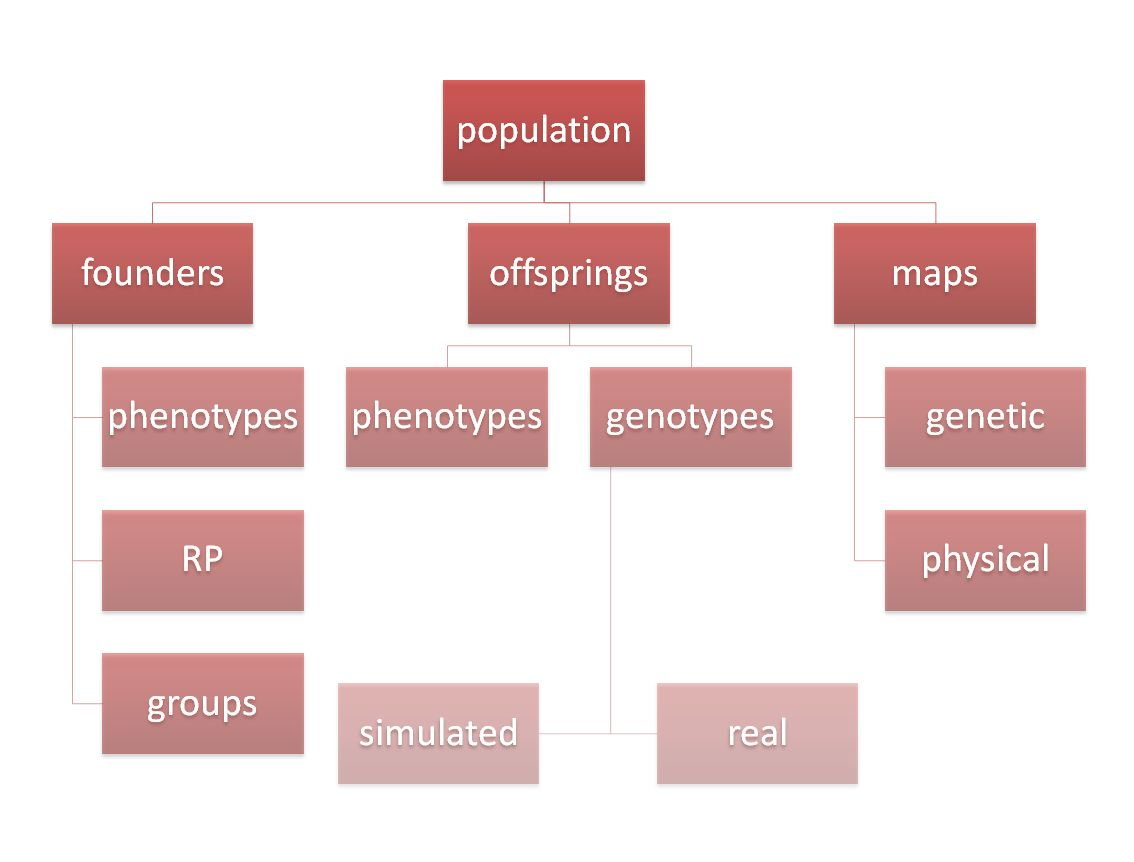
\includegraphics[scale=0.22]{population.jpg}
 \end{multicols}

\newpage
\section{Basic workflow}
\subsection{Loading data into workflow}
\subsubsection{readFiles function}
If data is formatted as specified in chapter 2 and files are having default names, you just have to type: 
\begin{Schunk}
\begin{Sinput}
> population <- readFiles(founders_groups = c(0, 0, 1, 1))
\end{Sinput}
\end{Schunk}
 into Rgui (make sure your working directory is the one containing data files) and it's all done. Parameter founders\_groups specifies in which column of parental file which parent is. Eg. you measured gene expression of both parents twice. Results for one of those are in first two columns, for the other - in following two. Then your function call will look exactly like one given above. 
If you don't like words founders, offspring and map and would like to use more friendly parents, children and treasure\_map instead, just type:
\begin{Schunk}
\begin{Sinput}
> population <- readFiles(offspring = "children", founders = "parents", map = "treasure_map", 
+     founders_groups = c(0, 0, 1, 1))
\end{Sinput}
\end{Schunk}
Function will then look for eg genetic map in file treasure\_map\_genetic.txt.
\subsubsection{createPopulation function}
Loading data from files is not always the best idea. Imagine you loaded your data into R already, for example to normalize it. Saving it back to disk and reading again into R means wasting your time. In this case you can use createPopulation function:
\begin{Schunk}
\begin{Sinput}
> population <- createPopulation(offspring_phenotypes, founders, founders_groups, offspring_genotypes, 
+     maps_genetic, maps_physical)
\end{Sinput}
\end{Schunk}
just listing objects that contain phenotype, genotype data and maps. For example if you have phenotype matrix called phenotypes for both founders(columns 1-4) and offspring(5-100) you can load that into population object using:
\begin{Schunk}
\begin{Sinput}
> population <- createPopulation(phenotypes[, 1:4], phenotypes[, 5:100], c(0, 0, 1, 1))
\end{Sinput}
\end{Schunk}
\subsection{Rank product analysis}
\subsubsection{Introduction}
Rank Product \citep{Hong:2006} is a powerful method to detect genes showing differential expression, especially in microarray experiments (citation). As so, it fits our needs perfectly and that's why it's incorporated into our workflow. For vast majority of the cases user just has to specify parental groups. This means providing function with a vector of 0s and 1s, specifying for each column of parental phenotype file which parent data does it contain. E.g. we measured both parents twice and first two columns contain information about first parent and other two about second. Then parental groups should be c(0,0,1,1) and function should be called: >  \$ population <- preprocessData(population,c(0,0,1,1))

{\noindent}If you're more experienced user and would like to provide RP function with additional parameters, it's possible. Just provide preprocessData funtion with them and they will be send directly to RP function. For further information see help files of RP and preprocessData functions.
\subsubsection{Example of function call}
\begin{Schunk}
\begin{Sinput}
> population <- findDiffExpressed(population)
\end{Sinput}
\end{Schunk}
\subsection{toGenotypes function}
After RankProduct analysis is done, it's time for magic to happen,  very essence of this package - creating genetic map out of gene expression data. If you're dataset come from experiment using of most common experimental breeding schemes - Recombinant Inbreed Lines, F2 or Back Cross, you should use corresponding set of parameters, described in section 3.4. If your breeding scheme is different, you will find all necessary information in sections 3.5 - 3.8.
\subsection{Preoptimized parameters for most common experimental crosses}
\subsubsection{Introduction}
We prepared preoptimized sets for most common experimental breeding schemes - Recombinant Inbreed Lines, F2 or Back Cross. You can just select one corresponding to your dataset, copy/paste it into R and everything is done for you. You still may be curious what exactly is happening and/or modify given sets to better suit your needs (e.g. more strict selection of the markers).
\subsubsection{Example of function call}
\subsection{Selecting appriopriate markers}
First step in toGenotypes analysis is selecting appropriate markers. Those are ones clearly differentially expressed between the parents. And having results from rank product you just have to specify p-value that determines whether difference in expression is significant(parameter threshold, default - 0.05). Normally it's 0.05 or 0.01. If you want to use all of your markers use threshold 0.5. Using any value above that will cause duplications (genes will be selected both as up- and down-regulated).
\subsection{Splitting selected markers} 
{\noindent}Once the appropriate markers are selected, they have to undergo splitting procedure, which means gene expression values are either assigned as 0 or 1, depending on which parent they come from. There are two methods to do so, as listed below.
\subsubsection{Parental mean splitting}
\blindtext
\subsubsection{EM splitting}
\blindtext
\subsection{Filtering markers}
\blindtext
\subsection{Cross object}
\blindtext[2]
\subsubsection{Creating cross object}
\blindtext
\subsubsection{Forming linkage groups and \\* ordering markers}
\blindtext
\subsubsection{Augmenting cross object}
\blindtext

\newpage
\section{Advanced options/modifications}

\subsection{Using data files with different \\* structure}
\blindtext
\subsection{Rank product analysis}
\blindtext
\subsection{Uncommon types of crosses}
\blindtext
\subsection{Modifying splitting options}
\blindtext
\subsection{Filtering markers}
\blindtext
\subsection{Cross object}
\blindtext
\subsubsection{Forming linkage groups and \\* ordering markers}
\blindtext
\subsubsection{Post-processing of cross object}
\blindtext

\newpage
\section{Built-in plotting routines}
\subsection{plotChildrenExpression}
\blindtext[2]
\subsection{plotParentalExpression}
\blindtext[2]
\subsection{plotMapComparison}
\blindtext[2]
\subsection{plotMarkerDistribution}
\blindtext[2]
\newpage
\section{Big datasets}

\subsection{Problematic handling of big data by R}
\blindtext
\subsection{C preprocessing}
\blindtext
\subsection{Other solutions}
\blindtext

\newpage
\section{Package development \& collaboration}
\newpage
\section{References}
\bibliographystyle{plainnat}
\bibliography{manual}
\end{document}
